%---------- Inleiding ---------------------------------------------------------

\section{Introductie}%
\label{sec:introductie}
\noindent
De meestgekende nieuwsbronnen proberen al lange tijd objectief en feitelijk te zijn, om informatie vanuit eenzelfde perspectief en met een vergelijkbare boodschap over te brengen. Door het hoogtepunt van de dag te abstraheren tot een uniek AI-gegenereerd kunstwerk, kan er worden geëxperimenteerd met de grenzen van de menselijke perceptie en kunst. \\
\noindent
Mijn toegepaste onderzoek richt zich op het ontwikkelen van een applicatie die kunstwerken genereert op basis van het dagelijkse hoogtepunt, waarvoor gegevens zullen worden verzameld door het 'scrapen' van nieuwswebsites en socialmediaplatformen.
Deze zal een kunstwerk genereren met behulp van één of meerdere deep learning modellen. \\
\noindent
Het doel is om te onderzoeken of AI al geavanceerd genoeg is om kunstwerken te creëren die niet van echt te onderscheiden zijn. Dit zal gebeuren met behulp van een turing test die zal bevestigen of het kunstwerk al dan niet geïdentificeerd wordt als AI-gegenereerd. \\
\noindent
Dit onderzoek kan interessante inzichten opleveren in de relatie tussen kunst, technologie en de samenleving.

%---------- Stand van zaken ---------------------------------------------------

\section{Literatuurstudie}%
\subsection{Wat is webscraping?} 
\noindent
Webscraping is een term die gebruikt wordt voor het extraheren van inhoud van websites om het te importeren in lokale opslag zoals een database of CSV bestand.  \autocite{Salem2020} \\
\noindent
Websites kunnen ervoor kiezen om een \emph{robots.txt} (\ref{fig:robotstxt}) in de root van hun filesystem te plaatsen. Binnen deze tekstfile kunnen ze beschrijven welke routes gescraped mogen worden. \autocite{GoogleDocs} \\
\begin{center}
    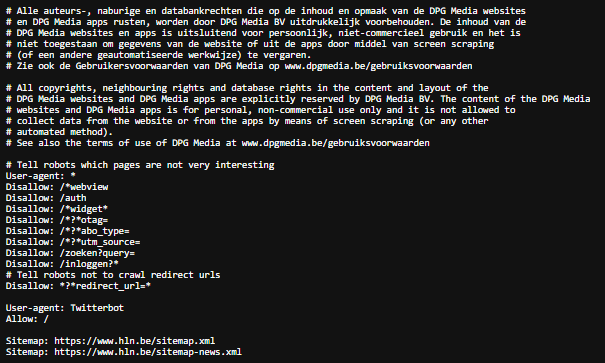
\includegraphics[width = 3in]{robotstxt_hln}
    \captionof{figure}{voorbeeld: www.hln.be/robots.txt}
    \label{fig:robotstxt}
\end{center}

\subsection{Wat is DALL-E (2)?}

\noindent
DALL-E is een AI software ontwikkeld door openAI dat beelden creëert uit tekstuele beschrijvingen, ook wel \emph{prompts} genoemd. Het gebruikt een versie met 12 miljard parameters van het GPT-3 Transformer-model om natuurlijke taalinvoer te interpreteren en overeenkomstige beelden te genereren. In april 2022 heeft OpenAI DALL-E 2 gelanceerd, ontwikkeld om meer realistische foto's met hogere resolutie te kunnen genereren. \\
 \autocite{DallEWikipediaNL}  \autocite{DallEWikipediaEN}\\

\noindent
DALL-E 2 is bovendien getrained met behulp van 650 milioen tekstinputs gescraped van het internet. \autocite{Borji2022} \\

\noindent
DALL-E 2 is niet open source maar kun je gebruiken aan de hand van de openAI API.  \\
\subsection{Wat is Stable Diffusion?}
\noindent
Stable Diffusion is een deep learning, tekst-naar-beeld model uitgebracht in 2022. In tegenstelling tot DALL-E (2) is Stable Diffusion getrained aan de hand van een diepe generatieve neurale netwerk.
\autocite{StableDifWikipediaEN}

Stable Diffusion is open source en kun je lokaal draaien op een computer met een GPU.



%---------- Methodologie ------------------------------------------------------
\section{Methodologie}%
\label{sec:methodologie}
\noindent
\textbf{Inleiding} \\
Het toegepast onderzoek begint 2 maart 2023 en zal beëindigd worden voor 28 mei 2023. \\

\noindent
\textbf{Fase 1: Realiseren van een scraper} \\
Om de data te bekomen van de verschillende soorten websites of social-media platformen zal er een web scraper worden gemaakt. Deze scraper zal ontwikkeld worden in python met behulp van een externe library \emph{BeautifulSoup}.

\noindent
Doordat de presentatie van de verschillende artikelen kunnen verschillen in taal en structuur, zal de scraper een algoritme implementeren die het mogelijk maakt om op een uniforme manier verschillende websites te scrapen. \\

\noindent
\textbf{Fase 2: Data verwerken en analyseren} \\
Tijdens de tweede fase zullen we onderzoeken op welke manier we de bekomen data uit voorgaande fase kunnen analyseren en sorteren. \\ \\
\noindent
Het zal belangrijk zijn om rekening te houden met de volgende vragen: 
\begin{itemize}
    \item Wat zijn de te extraheren kernzaken?
    \item Wat is het sentiment van de dag? 
    \item Welke topic komt het vaakst voor?
    \item Op basis van welke gegevens kunnen we de artikels sorteren? 
\end{itemize}

\noindent
Nadat er een gepaste methode wordt gevonden om dit te realiseren, zal deze ook geïmplementeerd worden. Op deze manier kunnen we steeds het belangrijkste artikel van de dag eruit halen. \\

\noindent
\textbf{Fase 3: Kunstwerk genereren} \\
Nu dat we weten uit de vorige fase wat het hoogtepunt van de dag was. Kunnen we hierop een kunstwerk laten genereren. \\
Hiervoor zal er gebruik gemaakt worden van een of meerdere deep learning modellen DALL-E 2 en/of Stable Diffusion die de kerntekst van een artikel zal omvormen tot een foto. \\

\noindent
\textbf{Fase 4: Turing test} \\ 
In de vierde fase van dit onderzoek willen we bepalen of de AI-gegenereerde kunstwerken van DALL-E 2 en/of Stable Diffusion niet van echt te onderscheiden zijn. We zullen hiervoor een Turing test uitvoeren. Een groep van 10 tot 20 personen krijgt twee sets van vijf kunstwerken te zien, waarvan er één AI-gegenereerd is en de andere vier door mensen zijn gemaakt. De deelnemers weten niet welk kunstwerk door de AI is gegenereerd. Vervolgens worden de deelnemers gevraagd om aan te geven welk kunstwerk zij denken dat door de AI is gegenereerd. Deze test zal helpen om te bepalen of de AI-gegenereerde kunstwerken van voldoende kwaliteit zijn om door mensen als 'echt' te worden ervaren. Op basis van de resultaten van de Turing test kan worden bepaald of de AI-gegenereerde kunstwerken van voldoende kwaliteit zijn om te worden beschouwd als volwaardige kunstwerken.

%---------- Verwachte resultaten ----------------------------------------------
\section{Verwacht resultaten}%
\label{sec:verwachte_resultaten}
\noindent
Het verwachte resultaat van het project is een goed functionerende applicatie die dagelijks een kunstwerk kan genereren op basis van het hoogtepunt van de dag.
\noindent
Op 27 oktober, toen Marokko won van België tijdens de WK kon het hoogtepunt in België \emph{'Riots in Brussels after soccer game, painting'} geweest zijn. Hieronder vindt u enkele voorbeelden die gegenereerd zijn met behulp van DALL-E 2 op basis van deze tekstinput. \\


\noindent
\begin{tabular}{llll}
    \label{fig:examples}
    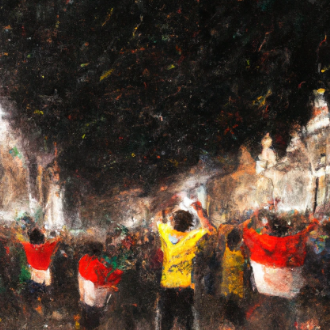
\includegraphics[width = 1.5in]{rellen_1.png} &
    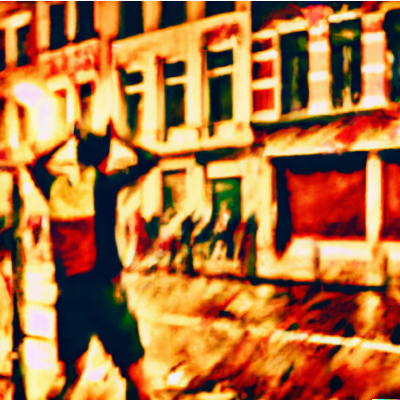
\includegraphics[width = 1.5in]{rellen_2.png} \\
    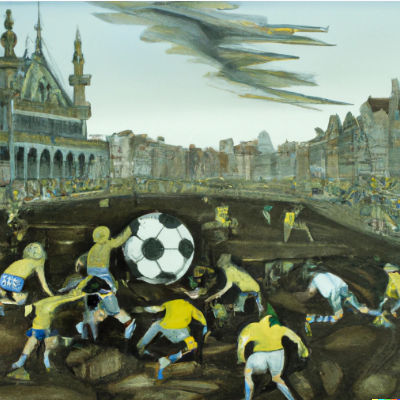
\includegraphics[width = 1.5in]{rellen_3.png} &
    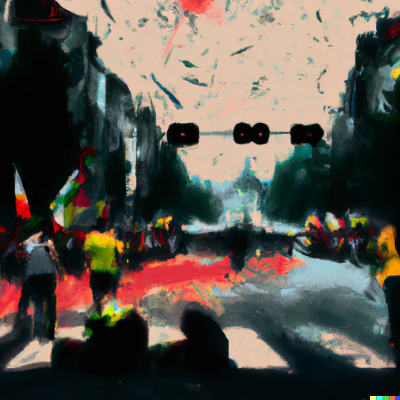
\includegraphics[width = 1.5in]{rellen_4.png}
\end{tabular} \\
\noindent
Daarnaast zal de Turing test uitwijzen of de gegenereerde kunstwerken geavanceerd genoeg zijn om te kunnen worden onderscheiden van kunstwerken die door mensen zijn gemaakt.
\noindent
Een voorbeeld van het resultaat van het project zou bijvoorbeeld kunnen zijn dat op een dag het hoogtepunt een artikel is over een nieuwe doorbraak in de gezondheidszorg. De applicatie zal dan op basis van de tekst van dat artikel een kunstwerk genereren dat hierbij past. In de verwachte resultaten zou dan bijvoorbeeld een afbeelding kunnen worden opgenomen van het gegenereerde kunstwerk op basis van het artikel over de gezondheidsdoorbraak inclusief 4 bestaande kunstwerken rond hetzelfde thema. Indien de X-aantal deelnemers  20\% juist scoren dan is de turing test geslaagd.

